% Source printed pp. 130-135, physical PDF pp. 138-143.
\section{等价关系与群胚}\label{src:4.4-section}
\begin{epigraph}
不同的人在不同的时期, 会为了不同的目的而使用不同的技巧.
\epigraphauthor{Serge Lang}
\end{epigraph}
我们证明, 等价关系和群胚的商可以构造为代数叠和代数空间 (定理~\bookref{4.4.13}). 此外, 代数空间或代数叠的任意呈示都诱导概形的等价关系或群胚. 等价关系和群胚不仅提供了构造代数空间与代数叠的有效方法, 也提供了理解这些对象的另一种方式.
\subsection{定义}\label{src:4.4.1-subsection}
\begin{definition}\label{src:4.4.1}
概形的\newterm{平展群胚}{étale groupoid} (相应地, \newterm{光滑群胚}{smooth groupoid}) 是两个概形 $U$ 和 $R$, 配备称为源的平展 (相应地, 光滑) 态射 $s:R\to U$, 称为靶的平展 (相应地, 光滑) 态射 $t:R\to U$, 以及满足下述条件的复合态射 $c:R\times_{s,U,t}R\to R$:
\begin{enumerate}[(1)]
\item (结合律) 下图交换:
\[
\begin{tikzcd}
R\times_{s,U,t}R\times_{s,U,t}R\arrow[r,"c\times\id"]\arrow[d,"\id\times c"']&R\times_{s,U,t}R\arrow[d,"c"]\\
R\times_{s,U,t}R\arrow[r,"c"']&R,
\end{tikzcd}
\]
\item (单位) 存在称为单位的态射 $e:U\to R$, 使下列图交换:
\[
\begin{tikzcd}[column sep=small]
{}&U\arrow[dl,"\id"']\arrow[d,"e"]\arrow[dr,"\id"]&{}\\
U&R\arrow[l,"s"]\arrow[r,"t"']&U
\end{tikzcd}
\qquad
\begin{tikzcd}[column sep=small]
R\arrow[r,"{(e\circ s,\id)}"]\arrow[dr,"\id"']&R\times_{s,U,t}R\arrow[d,"c"]&R\arrow[l,"{(e\circ t,\id)}"']\arrow[dl,"\id"]\\
{}&R,&{}
\end{tikzcd}
\]
\item (逆元) 存在称为逆元的态射 $i:R\to R$, 使下列图交换:
\[
\begin{tikzcd}[column sep=small]
R\arrow[r,"i"]\arrow[dr,"s"']&R\arrow[r,"i"]\arrow[d,"t"]&R\arrow[dl,"s"]\\
{}&U&{}
\end{tikzcd}
\qquad
\begin{tikzcd}[column sep=small]
R\arrow[r,"s"]\arrow[d,"{(i,\id)}"']&U\arrow[d,"e"]\\
R\times_{s,U,t}R\arrow[r,"c"']&R
\end{tikzcd}
\qquad
\begin{tikzcd}[column sep=small]
R\arrow[r,"t"]\arrow[d,"{(\id,i)}"']&U\arrow[d,"e"]\\
R\times_{s,U,t}R\arrow[r,"c"']&R.
\end{tikzcd}
\]
\end{enumerate}
我们常常滥用记号, 将这些数据简记为 $s,t:R\rightrightarrows U$.

若 $(s,t):R\to U\times U$ 是单态射, 则称 $s,t:R\rightrightarrows U$ 是\newterm{平展等价关系}{étale equivalence relation} (相应地, \newterm{光滑等价关系}{smooth equivalence relation}).

若 $U$ 和 $R$ 是代数空间, 且源, 靶与复合都是代数空间的态射, 就得到代数空间的平展 (相应地, 光滑) 群胚的概念, 以及代数空间的平展 (相应地, 光滑) 等价关系的概念.
\end{definition}
概形的群胚由 \cite[Exp. V]{SGA3I} 引入.
\begin{remark}[关系]\label{src:4.4.2}
可以将 $R$ 看作 $U$ 上的关系概形: 点 $r\in R$ 指定点 $s(r),t(r)\in U$ 之间的关系, 有时记为 $r:s(r)\to t(r)$. 对于每个概形 $T$, 态射 $R(T)\rightrightarrows U(T)$ 定义集合的群胚, 即存在复合映射 $R(T)\times_{s,U(T),t}R(T)\to R(T)$, 满足类似于定义~\bookref{4.4.1}(1)--(3) 的公理. 可将元素 $r\in R(T)$ 看作指定 $u,v\in U(T)$ 之间的关系 $r:u\to v$. 复合态射将关系 $r:u\to v$ 与 $r':v\to w$ 复合为关系 $r'\circ r:u\to w$, 单位态射将 $u\in U(T)$ 送到 $\id:u\to u$, 逆元态射将 $r:u\to v$ 送到 $r^{-1}:v\to u$. 当 $R\rightrightarrows U$ 是等价关系时, 态射 $R(T)\to U(T)\times U(T)$ 单射, $U(T)$ 的任意两个元素之间至多有一个关系.
\end{remark}
群胚的典型例子来自群作用.
\begin{example}[群作用]\label{src:4.4.3}
若 $G\to S$ 是平展 (相应地, 光滑) 群概形, 乘法为 $m:G\times_S G\to G$, 并通过 $\sigma:G\times U\to U$ 作用于 $S$ 上的概形 $U$, 则
\[
p_2,\sigma:G\times_S U\rightrightarrows U
\]
是概形的平展 (相应地, 光滑) 群胚. 逆元 $G\times_S U\to G\times_S U$ 由 $(g,u)\mapsto(g^{-1},gu)$ 给出, 复合为
\[
\begin{aligned}
(G\times_S U)\times_{p_2,U,\sigma}(G\times_S U)&\longrightarrow G\times_S U,\\
\bigl((g',u'),(g,u)\mid u'=gu\bigr)&\longmapsto(g'g,u).
\end{aligned}
\]
$G\times_S U$ 的 $T$-值点 $(g,u)$ 表示关系 $u\to gu$.

特殊情形 $U=S$ 定义群胚 $s,t:G\rightrightarrows S$, 其中两个箭头都等于结构态射 $G\to S$.
\end{example}
\begin{example}\label{src:4.4.4}
作为平展等价关系的一个有趣例子, 考虑 $\mathbb Z/2=\{\pm1\}$ 在 $\mathbb A^1$ 上的作用, 其作用映射 $\sigma:\mathbb Z/2\times\mathbb A^1\to\mathbb A^1$ 由 $-1\cdot x=-x$ 定义. 去掉原点稳定子中的非单位元素, 得到概形 $R=(\mathbb Z/2\times\mathbb A^1)\setminus\{(-1,0)\}$ 和等价关系 $p_2,\sigma:R\rightrightarrows\mathbb A^1$. 稍后将证明商 $X=\mathbb A^1/R$ 是代数空间, 但不是概形 (例~\bookref{4.9.2}).
\end{example}
% The source gives the example and its illustration the same number 4.4.4.
\addtocounter{theorem}{-1}
\begin{figure}[H]
\centering% Diagram 4.4.4: preserve both components, the deleted point and the red images.
\begin{tikzcd}[column sep=large,row sep=1.8em]
R=(\mathbb Z/2\times\mathbb A^1)\setminus\{(-1,0)\}\arrow[d]&
{\begin{tikzpicture}[baseline=-3pt,x=1cm,y=1cm,font=\small]
\draw[line width=.7pt] (-1.65,.22)--(1.65,.22);
\draw[line width=.7pt] (-1.65,0)--(1.65,0);
\fill[white] (0,0) circle (2.1pt);
\draw (0,0) circle (2.1pt);
\fill[red] (.9,0) circle (2pt);
\node[red,below] at (.9,0) {$x$};
\node[red,anchor=west] (unit) at (1.7,.55) {单位截面};
\draw[red,->] (unit.west)--(1.62,.24);
\end{tikzpicture}}\arrow[d,shift right=3pt,"p_2"']\arrow[d,shift left=3pt,"\sigma"]\\
\mathbb A^1&
{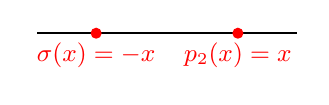
\begin{tikzpicture}[baseline=-3pt,x=1cm,y=1cm,font=\small]
\draw[line width=.7pt] (-1.65,0)--(1.65,0);
\fill[red] (-.9,0) circle (2pt);
\fill[red] (.9,0) circle (2pt);
\node[red,below] at (-.9,0) {$\sigma(x)=-x$};
\node[red,below] at (.9,0) {$p_2(x)=x$};
\end{tikzpicture}}
\end{tikzcd}

\caption{商 $X=\mathbb A^1/R$ 看起来像 $\mathbb A^1_{\mathbb R}$, 但原点的剩余域为 $\mathbb C$.}\label{src:4.4.4-figure}
\end{figure}
\begin{example}[呈示诱导的群胚]\label{src:4.4.5}
设 $\mathcal X$ 是 Deligne--Mumford 叠 (相应地, 代数叠), $p:U\to\mathcal X$ 是平展 (相应地, 光滑) 呈示; 假设此态射不仅可表, 而且可由概形表出.

定义代数空间 $R:=U\times_{\mathcal X}U$ (若 $\mathcal X$ 的对角线可由概形表出, 则它是概形). 由纤维积的定义, $R$ 的 $T$-值点是三元组 $(u_1,u_2,\alpha)$, 其中 $\alpha:p(u_1)\to p(u_2)$ 是 $\mathcal X(T)$ 中的同构, 将其看作关系 $\alpha:u_1\to u_2$. 令源态射 $s=p_1:R\to U$ 为第一投影, 靶态射 $t=p_2:R\to U$ 为第二投影, 则复合态射可定义为 $R\times_{s,U,t}R\to U\times_{\mathcal X}U$, 将 $(\alpha_2:u_2\to u_3,\alpha_1:u_1\to u_2)$ 送到 $\alpha_2\circ\alpha_1:u_1\to u_3$. 这给出代数空间的平展 (相应地, 光滑) 群胚 $R\rightrightarrows U$ 的结构. 注意, 若 $\mathcal X$ 是代数空间, 则对角线 $\mathcal X\to\mathcal X\times\mathcal X$ 是单态射. 因而 $(s,t):R\to U\times U$ 是单态射, $R\rightrightarrows U$ 是概形的平展等价关系.

选取不同的呈示会得到不同的群胚, 它们在称为 \newterm{Morita 等价}{Morita equivalence} 的意义下等价. 虽然这是一个重要概念, 本书并不使用它.

若 $U\to[U/G]$ 是商叠的呈示, 则诱导的群胚恰好是上一例所讨论的 $p_2,\sigma:G\times_S U\rightrightarrows U$. 实际上, 存在自然等同 $U\times_{[U/G]}U\xrightarrow{\sim}G\times_S U$, 由 $u_1\times_g u_2\mapsto(g,u_2)$ 定义, 其中 $u_1\times_g u_2$ 是定义纤维积中元素的三元组 $(u_1=gu_2,u_2,g)$ 的简记. 类似地, $U\times_{[U/G]}U\times_{[U/G]}U\xrightarrow{\sim}G\times_S G\times_S U$ 由 $u_1\times_{g_1}u_2\times_{g_2}u_3\mapsto(g_1,g_2,u_3)$ 给出. 群胚中的各个投影映射可等同于群作用给出的映射:
\[
\begin{tikzcd}[row sep=large,column sep=large]
U\times_{[U/G]}U\times_{[U/G]}U\arrow[r,"\sim"]\arrow[d,shift right=8pt,"p_{12}"'{pos=.7}]\arrow[d,"p_{13}"{description,pos=.3}]\arrow[d,shift left=8pt,"p_{23}"{pos=.7}]&G\times_S G\times_S U\arrow[d,shift right=8pt,"\id\times\sigma"'{pos=.7}]\arrow[d,"m\times\id"{description,pos=.3}]\arrow[d,shift left=8pt,"p_{23}"{pos=.7}]\\
U\times_{[U/G]}U\arrow[r,"\sim"]\arrow[d,shift right=3pt,"p_1"']\arrow[d,shift left=3pt,"p_2"]&G\times_S U\arrow[d,shift right=3pt,"p_2"']\arrow[d,shift left=3pt,"\sigma"]\\
U\arrow[r,equal]\arrow[d]&U\\
{[U/G].}&{}
\end{tikzcd}
\]
\end{example}
\begin{exercise}\label{src:4.4.6}
证明存在等同
\[
\begin{aligned}
(U/[U/G])^n:=\underbrace{U\times_{[U/G]}\cdots\times_{[U/G]}U}_{n\text{ 次}}&\xrightarrow{\sim}G^{n-1}\times_S U,\\
u_1\times_{g_1}\cdots\times_{g_{n-1}}u_n&\longmapsto(g_1,\ldots,g_{n-1},u_n),
\end{aligned}
\]
其中 $u_i=g_i u_{i+1}$, 使忘掉第 $k$ 项的投影映射 $(U/[U/G])^{n+1}\to(U/[U/G])^n$ 等同于映射
\[
G^n\times U\longrightarrow G^{n-1}\times U,
\]
\[
(g_1,\ldots,g_n,u_{n+1})\longmapsto
\begin{cases}
(g_2,\ldots,g_n,u_{n+1})&k=1,\\
(g_1,\ldots,g_{k-2},g_{k-1}g_k,g_{k+1},\ldots,g_n,u_{n+1})&k=2,\ldots,n,\\
(g_1,\ldots,g_n,g_nu_{n+1})&k=n+1.
\end{cases}
\]
\end{exercise}
\begin{definition}[轨道与稳定子]\label{src:4.4.7}
设 $R\rightrightarrows U$ 是代数空间的光滑群胚, $x:\Spec k\to U$ 是域值点. $x$ 的稳定子 $G_x$ (或 $x$ 的自同构群 $\Aut(x)$) 定义为 $(s,t):R\to U\times U$ 沿 $(x,x):\Spec k\to U\times U$ 的纤维积. 轨道 $O(x)$ 定义为集合 $s(t^{-1}(x))\subseteq U$.
\end{definition}
\begin{remark}\label{src:4.4.8}
注意, 若群胚 $R\rightrightarrows U$ 来自代数叠的光滑呈示 $U\to\mathcal X$, 则 $x\in U(k)$ 的稳定子等同于其在 $\mathcal X(k)$ 中的像的稳定子. 另一方面, 轨道 $O(x)$ 是 $U$ 中在 $R$ 内存在关系 $x\xrightarrow{\sim}y$ 的点 $y$ 的集合, 等价地, 它是 $U$ 中在 $\mathcal X$ 内的像与 $x$ 的像同构的点 $y$ 的集合.
\end{remark}
\begin{exercise}[不重要]\label{src:4.4.9}
在定义~\bookref{4.4.1}~中, 证明单位态射和逆元态射唯一确定.
\end{exercise}
\subsection{群胚商的代数性}\label{src:4.4.2-subsection}
\begin{definition}[光滑群胚的商叠]\label{src:4.4.10}
设 $s,t:R\rightrightarrows U$ 是代数空间的光滑群胚. 定义 $[U/R]^{\mathrm{pre}}$ 为如下预叠: 对象是来自概形 $T$ 的态射 $T\to U$, 态射 $(a:S\to U)\to(b:T\to U)$ 是概形态射 $f:S\to T$ 和元素 $r\in R(S)$ 的数据, 满足 $s(r)=a$ 及 $t(r)=f\circ b$. 定义 $[U/R]$ 为 $[U/R]^{\mathrm{pre}}$ 在大平展拓扑 $\Sch_{\text{ét}}$ 中的叠化. 若 $R\rightrightarrows U$ 还是等价关系, 则 $[U/R]$ 同构于层 (习题~\bookref{4.4.12}), 记为 $U/R$.
\end{definition}
纤维范畴 $[U/R]^{\mathrm{pre}}(T)$ 是对象为 $U(T)$, 态射为 $R(T)$ 的群胚. 恒等态射 $\id:U\to U$ 定义映射 $U\to[U/R]^{\mathrm{pre}}$, 从而给出映射 $p:U\to[U/R]$.
\begin{exercise}[重要]\label{src:4.4.11}
推广习题~\bookref{3.4.37}, 证明若 $s,t:R\rightrightarrows U$ 是代数空间的光滑群胚, 则下列图为 Cartesian 图:
\[
\begin{tikzcd}
R\arrow[r,"s"]\arrow[d,"t"']\arrow[dr,phantom,"\square"]&U\arrow[d,"p"]\\
U\arrow[r,"p"']&{[U/R]}
\end{tikzcd}
\qquad\text{和}\qquad
\begin{tikzcd}
R\arrow[r,"{(s,t)}"]\arrow[d]\arrow[dr,phantom,"\square"]&U\times U\arrow[d,"p\times p"]\\
{[U/R]}\arrow[r,"\Delta"']&{[U/R]\times[U/R].}
\end{tikzcd}
\]
\end{exercise}
\begin{exercise}\label{src:4.4.12}
设 $R\rightrightarrows U$ 是代数空间的光滑群胚. 证明 $[U/R]$ 等价于层当且仅当 $R\rightrightarrows U$ 是等价关系.
\end{exercise}
\begin{theorem}[群胚商的代数性]\label{src:4.4.13}
\begin{enumerate}[(1)]
\item 若 $R\rightrightarrows U$ 是代数空间的平展 (相应地, 光滑) 群胚, 则 $[U/R]$ 是 Deligne--Mumford 叠 (相应地, 代数叠), $U\to[U/R]$ 是平展 (相应地, 光滑) 呈示.
\item 若 $R\rightrightarrows U$ 是概形的平展等价关系, 则 $U/R$ 是代数空间, $U\to U/R$ 是平展呈示.
\end{enumerate}
\end{theorem}
\begin{remark}\label{src:4.4.14}
在推论~\bookref{5.5.12}~中, 将证明代数空间的平展等价关系的商 $U/R$ 实际上也是代数空间. 这说明, 考虑在平展局部为代数空间的层不会得到新的代数几何对象. 此结果推迟到 \S\bookref{5.5}, 因为证明 $U/R$ 的对角线可由概形表出需要更多工作. 更一般地, 若 $R\rightrightarrows U$ 是代数空间的 fppf 群胚 (相应地, fppf 等价关系), 则 $[U/R]$ 是代数叠 (相应地, $U/R$ 是代数空间); 见推论~\bookref{7.3.6}.
\end{remark}
\begin{proof}
对于定理~\bookref{4.4.13}(1), 我们证明 $U\to\mathcal X:=[U/R]$ 满射, 光滑且可表. 设 $T\to\mathcal X$ 是来自概形 $T$ 的态射. 由 $[U/R]$ 定义为 $[U/R]^{\mathrm{pre}}$ 的叠化, 存在平展覆盖 $T'\to T$ 和交换图
\[
\begin{tikzcd}
T'\arrow[r]\arrow[d]&U\arrow[d]\\
T\arrow[r]&\mathcal X.
\end{tikzcd}
\]
在预叠的交换立方体
\begin{equation}\label{src:4.4.15}
\begin{tikzcd}[row sep=1.1em,column sep=1.4em]
{}&U_{T'}\arrow[rr]\arrow[dl]\arrow[dd]&{}&T'\arrow[dl]\arrow[dd]\\
R\arrow[rr]\arrow[dd]&{}&U\arrow[dd]&{}\\
{}&U_T\arrow[rr]\arrow[dl]&{}&T\arrow[dl]\\
U\arrow[rr]&{}&\mathcal X,&{}
\end{tikzcd}
\end{equation}
中, 前, 后, 上, 下四个方块都是 Cartesian 方块. 需要证明层 $U_T$ 是代数空间, 但这并不困难: $U_{T'}$ 是概形, $U_{T'}\to U_T$ 是可由概形表出的满射平展态射 (因为它是 $T'\to T$ 的基变换). 由于 $R\to U$ 满射且平展 (相应地, 光滑), $U_{T'}\to T'$ 亦然, 因而由平展下降, $U_T\to T$ 也如此.

对于定理~\bookref{4.4.13}(2), 已知 $U/R$ 是层, $U\to U/R$ 满射, 平展且可表. 需要证明 $U\to U/R$ 可由概形表出. 只需证明 $X$ 的对角线可由概形表出; 见推论~\bookref{4.2.3}(1). 设 $T\to X\times X$ 是来自概形的态射, 利用 Cartesian 立方体
\begin{equation}\label{src:4.4.16}
\begin{tikzcd}[row sep=1.1em,column sep=1.4em]
{}&Q_{T'}\arrow[rr]\arrow[dl]\arrow[dd]&{}&T'\arrow[dl]\arrow[dd]\\
R\arrow[rr]\arrow[dd]&{}&U\times U\arrow[dd]&{}\\
{}&Q_T\arrow[rr]\arrow[dl]&{}&T\arrow[dl]\\
X\arrow[rr]&{}&X\times X,&{}
\end{tikzcd}
\end{equation}
定义 $Q_T$ 和 $Q_{T'}$. 由于 $R\to U\times U$ 局部拟有限且分离, $Q_{T'}\to T'$ 亦然. fppf 层成为概形的下降判据 (命题~\bookref{3.3.17}) 蕴涵 $Q_T$ 是概形.
\end{proof}
\begin{remark}[再论商叠]\label{src:4.4.17}
由此可见, 商叠的代数性 (\bookref{4.1.10}) 中群概形 $G\to S$ 仿射的假设, 对于商叠 $[X/G]$ 或分类叠 $BG$ 的代数性并非必要.
\end{remark}
\begin{exercise}[重要]\label{src:4.4.18}
证明若 $\mathcal X$ 是代数叠 (相应地, 代数空间), $U\to\mathcal X$ 是光滑呈示, 则 $\mathcal X$ 同构于平展群胚 (相应地, 等价关系) $R\rightrightarrows U$ 的商叠 $[U/R]$ (相应地, 商层 $U/R$), 其中 $R=U\times_{\mathcal X}U$.
\end{exercise}
\subsection{诱导呈示与切片呈示}\label{src:4.4.3-subsection}
这里介绍两种从已有呈示构造新呈示的有用技巧.

首先, 考虑商叠 $\mathcal X=[X/H]$, 其中 $H$ 是作用于 $k$ 上概形 $X$ 的光滑仿射代数群. 若另一个群 $G$ 包含 $H\subseteq G$ 作为子群, 则 $H$ 通过 $h\cdot(g,x)=(gh^{-1},hx)$ 自由作用于 $G\times X$, 可以定义商代数空间
\[
G\times^H X:=(G\times X)/H,
\]
它有时称为 \newterm{Borel 构造}{Borel construction}. 目前只知道它是可由代数叠表出的层 (定理~\bookref{4.4.13}(1)), 但推论~\bookref{4.6.8}~将说明它实际上是代数空间. (若 $H$ 是有限抽象群, 则定理~\bookref{4.4.13}(2) 已经蕴涵它是代数空间.) 无论如何, $G$ 通过 $g\cdot(g',x)=(gg',x)$ 作用于 $G\times^H X$.
\begin{exercise}\label{src:4.4.19}
证明 $[X/H]\cong[(G\times^H X)/G]$.
\end{exercise}
商呈示 $[G\times^H X/G]$ 称为\newterm{诱导呈示}{induced presentation}.

第二种技巧称为\newterm{群胚切片}{slicing a groupoid}. 设 $U\to\mathcal X$ 是代数叠的光滑呈示, 对应的群胚为 $s,t:R=U\times_{\mathcal X}U\rightrightarrows U$. 若 $g:U'\to U$ 是态射, 则将 $R\rightrightarrows U$ 沿 $U'\to U$ 的限制定义为群胚 $R|_{U'}\rightrightarrows U'$, 其中 $R|_{U'}$ 由纤维积
\[
\begin{tikzcd}
R|_{U'}\arrow[r,"{(t',s')}"]\arrow[d]\arrow[dr,phantom,"\square"]&U'\times U'\arrow[d]\\
R\arrow[r,"{(t,s)}"']&U\times U
\end{tikzcd}
\]
定义.
\begin{exercise}\label{src:4.4.20}
\begin{enumerate}[(a)]
\item 证明 $R|_{U'}$ 嵌入 Cartesian 图
\[
\begin{tikzcd}[column sep=large]
R|_{U'}\arrow[r]\arrow[d]\arrow[dr,phantom,"\square"]&R\times_{s,U}U'\arrow[r]\arrow[d]\arrow[dr,phantom,"\square"]&U'\arrow[d,"g"]\\
U'\times_{U,t}R\arrow[r]\arrow[d]\arrow[dr,phantom,"\square"]&R\arrow[r,"s"]\arrow[d,"t"]\arrow[dr,phantom,"\square"]&U\arrow[d]\\
U'\arrow[r,"g"']&U\arrow[r]&{[U/R].}
\end{tikzcd}
\]
\end{enumerate}
再假设 $U'\times_{U,t}R\to R\xrightarrow{s}U$ 平展 (相应地, 光滑).
% Preserve the source's switch from (a) to (2)-(4).
\begin{enumerate}[(1)]\setcounter{enumi}{1}
\item 证明 $R|_{U'}\rightrightarrows U'$ 是平展 (相应地, 光滑) 群胚.
\item 证明存在开浸入 $[U'/R|_{U'}]\to[U/R]$.
\item 证明 $[U'/R|_{U'}]\to[U/R]$ 是同构, 当且仅当对于每个点 $u\in U$, 都存在点 $u'\in U$ 以及 $R$ 中的关系 $u\to g(u')$.
\end{enumerate}
\end{exercise}
\begin{exercise}[再论椭圆曲线的模]\label{src:4.4.21}
考虑习题~\bookref{4.1.21}~中的椭圆曲线模叠 $\mathcal M_{1,1}\cong[(\mathbb A^2\setminus V(\Delta))/\mathbb G_m]$, 其中 $k$ 是满足 $\operatorname{char}(k)\ne2,3$ 的域, $\Delta=4a^3+27b^2$ 是判别式 ($a$ 和 $b$ 为 $\mathbb A^2$ 上的坐标). 沿闭浸入 $V(\Delta-1)\hookrightarrow\mathbb A^2\setminus V(\Delta)$ 作切片, 证明 $\mathcal M_{1,1}\cong[V(\Delta-1)/\mu_{12}]$ 是仿射概形对有限群的商.
\end{exercise}
